\section{Sombreamento parcial e diodos de bypass}\label{sec:sombra}

Arquivos: \arq{painel/painel_sombreado.m}, \arq{painel/residuo_painel.m},
\arq{cenarios/aplicar_sombras.m}. Aqui o m\'odulo deixa de ser um bloco \'unico e vira tr\^es
subm\'odulos em s\'erie, cada um com a sua irradi\^ancia.

\subsection{A f\'isica}

Em s\'erie, todos os subm\'odulos conduzem a mesma corrente $I$ e as tens\~oes somam. Se um
subm\'odulo recebe pouca luz, n\~ao consegue gerar essa corrente; sem prote\c{c}\~ao seria for\c{c}ado
a tens\~ao negativa e esquentaria (ponto quente). O \textbf{diodo de bypass}, em antiparalelo,
conduz quando a tens\~ao do subm\'odulo cai para cerca de $-0{,}4$\,V: a corrente passa por ele e o
subm\'odulo sombreado deixa de contribuir com tens\~ao. O c\'odigo modela o bypass como um Schottky
($I_{0bp}=1{,}4\times10^{-6}$\,A, queda de $\sim$0,4\,V a 8\,A).

\begin{figure}[htbp]
\centering
\begin{circuitikz}[scale=0.85,transform shape]
  \foreach \y/\i in {0/1,2.8/2,5.6/3} {
    \draw (0,\y) -- (0,\y+0.6) to[battery2,l=$V_\i$] (0,\y+2.2) -- (0,\y+2.8);
    \draw (0,\y+0.6) -- (2.6,\y+0.6) to[D,l_=bypass $\i$] (2.6,\y+2.2) -- (0,\y+2.2);
  }
  \draw (0,8.4) to[short,-o] (0,8.9) node[above]{$+$};
  \draw (0,0) to[short,-o] (0,-0.5) node[below]{$-$};
  \node[font=\scriptsize,gray,anchor=west] at (5.2,4.7) {a mesma corrente $I$ atravessa os tr\^es};
  \node[font=\scriptsize,gray,anchor=west] at (5.2,4.2) {$V_{pv}=V_1+V_2+V_3$};
  \node[font=\scriptsize,gray,anchor=west] at (5.2,3.4) {o bypass fica em reverso};
  \node[font=\scriptsize,gray,anchor=west] at (5.2,2.9) {enquanto o subm\'odulo est\'a iluminado};
\end{circuitikz}
\caption{Tr\^es subm\'odulos em s\'erie, cada um com seu diodo de bypass em antiparalelo. Esquema conceitual.}
\label{fig:bypass}
\end{figure}

\subsection{As equa\c{c}\~oes}

O vetor de inc\'ognitas \'e $z=[I;\,V_{d,1};\dots;V_{d,N}]$, com $V_{d,j}$ a tens\~ao de jun\c{c}\~ao
do subm\'odulo $j$. Dado $V_{d,j}$, tudo no subm\'odulo \'e expl\'icito:
\begin{align}
I_{c,j}&=I_{pv,j}-I_{01}\big(e^{V_{d,j}/(a_1V_t)}-1\big)-I_{02}\big(e^{V_{d,j}/(a_2V_t)}-1\big)-\frac{V_{d,j}}{R_{p,j}}\\
V_j&=V_{d,j}-R_sI_{c,j}\\
I_{bp,j}&=I_{0bp}\big(e^{-V_j/V_{t,bp}}-1\big)
\end{align}
O sistema tem $N+1$ equa\c{c}\~oes:
\begin{align}
R_j&=I_{c,j}+I_{bp,j}-I=0 &&\text{(KCL: c\'elulas + bypass = corrente da fileira)}\\
R_{N+1}&=\textstyle\sum_jV_j-V_{pv}=0 &&\text{(KVL: a tens\~ao do terminal \'e a soma)}
\end{align}

\codigointeiro{painel/residuo_painel.m}{res\'iduo $R(z)$ e jacobiano anal\'itico $J=dR/dz$.}{lst:residuo}

\begin{logica}
\begin{enumerate}
\item \texttt{celula\_params} entrega, para cada subm\'odulo, $R_p$, $I_{pv}$, $I_{01}$, $I_{02}$ (um valor por
 elemento de $G$).
\item \texttt{Ic} \'e a corrente das c\'elulas; \texttt{Vj} a tens\~ao nos terminais do subm\'odulo;
 \texttt{Ibp} a do bypass. Se \texttt{Vj} \'e negativo, \texttt{exp(-Vj/Vt\_bp)} dispara e o bypass
 conduz muito.
\item \texttt{R} empilha as $N$ equa\c{c}\~oes de KCL e a de KVL.
\item \textbf{Jacobiano anal\'itico:} $\partial R_j/\partial I=-1$; $\partial R_j/\partial V_{d,j}=-g-h\,dV_j$
 (com $g=-dI_c/dV_d$, $h=-dI_{bp}/dV_j$, $dV_j=1+R_sg$); a \'ultima linha \'e $dV_j$ (derivada da soma de tens\~oes).
\end{enumerate}
\end{logica}

\subsection{Newton--Raphson com passo limitado}

\codigointeiro{painel/painel_sombreado.m}{corrente do m\'odulo sob sombra por Newton.}{lst:newton}

\begin{logica}
\begin{enumerate}
\item \textbf{Chute inicial.} Sem \emph{warm start}: $I_0=I_{pv,n}\min(G)/G_n$ e $V_d=V_{pv}/N+0{,}5V_t$. Com
 \emph{warm start}, usa-se a solu\c{c}\~ao do ponto anterior.
\item A cada itera\c{c}\~ao calcula-se $R$ e $J$; para se $\|R\|_\infty<10^{-9}$; sen\~ao $\Delta z=-J^{-1}R$.
\item \textbf{Limite de passo:} a corrente muda no m\'aximo 2\,A e cada $V_d$ no m\'aximo $2V_t$ por itera\c{c}\~ao.
 Sem isso, um passo grande de exponencial estoura (overflow).
\item M\'aximo de 60 itera\c{c}\~oes; se n\~ao convergir, avisa com \texttt{warning}.
\item Sa\'idas auxiliares (\texttt{sol.Vj}, \texttt{sol.Ibp}\ldots) servem aos testes de bypass.
\end{enumerate}
\end{logica}

\subsection{O que sai: curvas P-V com v\'arios picos}

O experimento E2 mede os picos de tr\^es cen\'arios do ZTP-160M a 25\,$^\circ$C:

\begin{resultado}
\small\centering
\begin{tabular}{@{}llccc@{}}
\toprule
Cen\'ario & Irradi\^ancia relativa & $V$ [V] & $P$ [W] & Global? \\ \midrule
Sem sombra & [1 1 1] & 19,57 & 160,5 & sim \\
1 subm\'odulo a 40\,\% & [1 1 0,4] & 12,68 & 103,8 & \textbf{sim} \\
1 subm\'odulo a 40\,\% & [1 1 0,4] & 20,69 & 70,2 & n\~ao \\
Degrad\^e 100/60/30\,\% & [1 0,6 0,3] & 5,80 & 47,3 & n\~ao \\
Degrad\^e 100/60/30\,\% & [1 0,6 0,3] & 13,08 & 65,9 & \textbf{sim} \\
Degrad\^e 100/60/30\,\% & [1 0,6 0,3] & 20,49 & 52,2 & n\~ao \\
\bottomrule
\end{tabular}
\end{resultado}

No caso de 1 subm\'odulo a 40\,\%, o pico mais pr\'oximo de $\Voc$ (20,7\,V, 70\,W) \'e local. Um
algoritmo que parta de $\Voc$ e suba a ladeira termina ali e perde 33\,W (32\,\%) em rela\c{c}\~ao ao
pico global de 12,7\,V. No degrad\^e, o global est\'a no meio. Os picos globais sombreados ficam
em 12,7 e 13,1\,V, perto da bateria de 12\,V, e outros ficam abaixo: por isso o conversor precisa
operar como buck \emph{e} como boost (D3).

\begin{figure}[htbp]
\centering
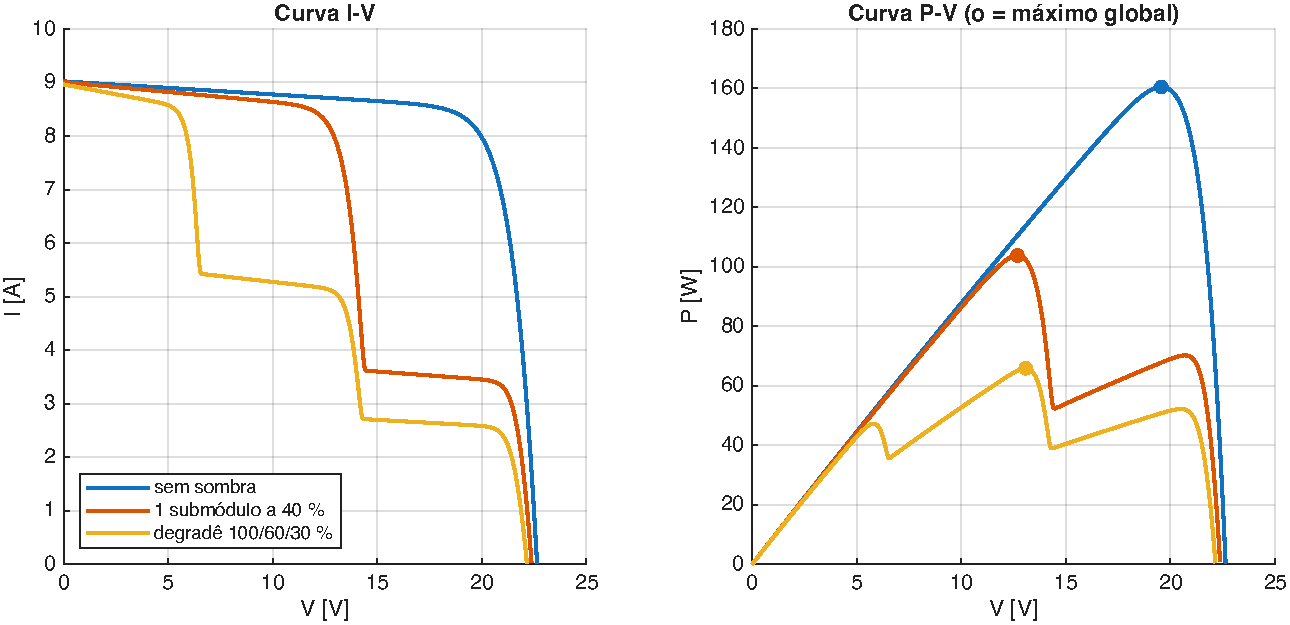
\includegraphics[width=0.92\linewidth]{e2_curvas_sombra.pdf}
\caption{E2. Curvas I-V e P-V do ZTP-160M sob tr\^es padr\~oes de sombra: aparecem de 1 a 3 picos.}
\label{fig:e2}
\end{figure}
